\documentclass[11pt]{article}

\usepackage{amsmath}
\usepackage{amssymb}
\usepackage[margin=0.68in]{geometry}
\usepackage{booktabs}
\usepackage{enumitem}
\usepackage{fancyhdr}
\usepackage{graphicx}
\usepackage[hidelinks]{hyperref}
\usepackage{listings}
\usepackage{microtype}
\usepackage{tabularx}
\usepackage{tikz}
\usepackage{titlesec}
\usepackage[table]{xcolor}
\usetikzlibrary{arrows.meta,positioning}
\graphicspath{{docs/lessons/assets/}{../assets/}}

\definecolor{AdkBlack}{gray}{0}
\definecolor{AdkDark}{gray}{0.20}
\definecolor{CodeGray}{gray}{0.96}
\hypersetup
{
    pdftitle={ADK Lesson 013: DHT11 Climate Sensor},
    pdfauthor={Kevin Shanahan},
    pdfsubject={Validated climate samples, scheduled DHT11 acquisition, and circuit-native evidence},
    pdflang={en-US}
}
\pagestyle{fancy}
\fancyhf{}
\lhead{\textsc{ADK Lesson 013}}
\rhead{DHT11 Climate Sensor}
\cfoot{\thepage}
\setlength{\headheight}{14pt}
\setlength{\parindent}{0pt}
\setlength{\parskip}{5pt}
\setlist{nosep,leftmargin=1.45em}
\titleformat{\section}{\Large\bfseries\color{AdkBlack}}{\thesection}{0.5em}{}
\titleformat{\subsection}{\large\bfseries\color{AdkBlack}}{\thesubsection}{0.5em}{}
\lstdefinestyle{adkcpp}
{
    language=C++,
    backgroundcolor=\color{CodeGray},
    basicstyle=\ttfamily\footnotesize,
    keywordstyle=\color{AdkBlack}\bfseries,
    commentstyle=\color{AdkDark},
    columns=fullflexible,
    keepspaces=true,
    showstringspaces=false,
    frame=single,
    rulecolor=\color{black!20},
    breaklines=true,
    tabsize=4
}
\newcommand{\checkbox}{\(\square\)}
\newcommand{\blank}[1]{\rule{#1}{0.4pt}}
\newcommand{\warningbox}[1]{%
  \begin{center}
  \fcolorbox{black}{white}{\parbox{0.91\linewidth}{\textbf{Safety checkpoint.} #1}}
  \end{center}}
\newcommand{\evidencebox}[1]{%
  \begin{center}
  \fcolorbox{black}{white}{\parbox{0.91\linewidth}{#1}}
  \end{center}}

\begin{document}

\begin{center}
  {\Huge\bfseries DHT11 Climate Sensor}\\[4pt]
  {\Large Separate transport, validity, freshness, and physical accuracy}\\[8pt]
  \textit{The RGB cadence reports software state; TP13 reveals the wire.}
\end{center}

\begin{tabularx}{\linewidth}{@{}>{\bfseries}l X >{\bfseries}l X@{}}
Lesson & 013 --- component & Time & 120--180 minutes\\
Prerequisites & Lessons 001--012 & Board & Arduino Mega 2560\\
Evidence & D5--D7 status indicator and TP13 & Status &
host verified; physical acceptance open\\
Safety & E1; USB-powered low-current circuit only\\
\end{tabularx}

\warningbox{Disconnect USB before wiring. Identify the exact bare sensor or
module before adding a DATA pull-up: many modules already contain one. Never
connect the DHT11 NC pin. Stop for heat, odor, resets, unstable power, a DATA
voltage outside the supply rails, or disagreement between the table and the
identified part. Remove USB power to stop the experiment.}

\section{Mission}

Build a scheduled climate observation path:

\[
\text{DHT11 at D22}\rightarrow\texttt{Dht11Sensor}\rightarrow
\texttt{ClimateSample}\rightarrow\text{D5--D7 status evidence}.
\]

The lesson deliberately does not add a display. Numeric presentation belongs
to lesson 014. Here the learner asks four narrower questions:

\begin{enumerate}
  \item Did the software acquire its pin resource?
  \item Did a bounded wire transaction complete?
  \item Did checksum and range validation accept the decoded sample?
  \item Is the last accepted sample still fresh under the lesson policy?
\end{enumerate}

Those claims are independent. A pulse train at TP13 does not establish climate
accuracy. A green indicator means the decoded sample is fresh and valid, not
that the sensor has been calibrated against a reference instrument.

\section{Composition and lifecycle}

\begin{center}
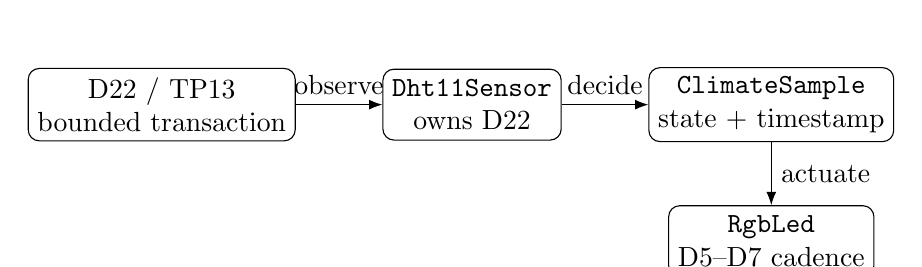
\begin{tikzpicture}[
    node distance=8mm and 11mm,
    box/.style={draw,rounded corners,minimum height=9mm,align=center},
    >=Latex]
  \node[box] (wire) {D22 / TP13\\bounded transaction};
  \node[box,right=of wire] (sensor) {\texttt{Dht11Sensor}\\owns D22};
  \node[box,right=of sensor] (sample) {\texttt{ClimateSample}\\state + timestamp};
  \node[box,below=of sample] (led) {\texttt{RgbLed}\\D5--D7 cadence};
  \draw[->] (wire) -- node[above]{observe} (sensor);
  \draw[->] (sensor) -- node[above]{decide} (sample);
  \draw[->] (sample) -- node[right]{actuate} (led);
\end{tikzpicture}
\end{center}

Construction is inert. \texttt{initialize()} validates and claims D22, leaves
the pulled-up DATA wire released as an input, and sets the sample to
\texttt{Unavailable}. Repeated initialization is harmless. A failed RGB
acquisition shuts the sensor down before setup returns.

\texttt{update(now)} schedules the next eligible transaction from caller
supplied time. It never uses an unbounded wait. An early call is a successful
no-op. \texttt{sample(now, freshFor)} reads state without touching hardware.
\texttt{shutdown()} releases DATA to high impedance, clears the snapshot,
releases the claim, and is idempotent. The destructor repeats that cleanup
safely.

\begin{lstlisting}[style=adkcpp]
void loop ()
{
    const adk::TimePoint     now         (millis ());
    const adk::Status        status      = observeClimate     (now);
    const adk::ClimateSample observation = decideClimateState (now);

    showClimateState (observation, now);
}
\end{lstlisting}

The canonical sketch additionally checks each status and halts with outputs
off if the evidence circuit itself fails.

\section{Parts and orientation}

\begin{tabularx}{\linewidth}{@{}l l X@{}}
\toprule
Quantity & Part & Requirement\\
\midrule
1 & Mega 2560 & USB powered\\
1 & DHT11 & exact bare part or documented module identified\\
1 & DATA pull-up & value from the identified part; omit if module supplies it\\
1 & common-cathode RGB LED & each die identified before wiring\\
3 & 330\,\(\Omega\) resistors & one for each RGB channel\\
1 & 0.1\,\(\mu\)F capacitor & across sensor VDD/GND when part guidance calls for it\\
1 & logic analyzer or oscilloscope & optional TP13 timing evidence\\
1 & multimeter & continuity, rail, and released-level checks\\
\bottomrule
\end{tabularx}

\begin{figure}[ht]
  \centering
  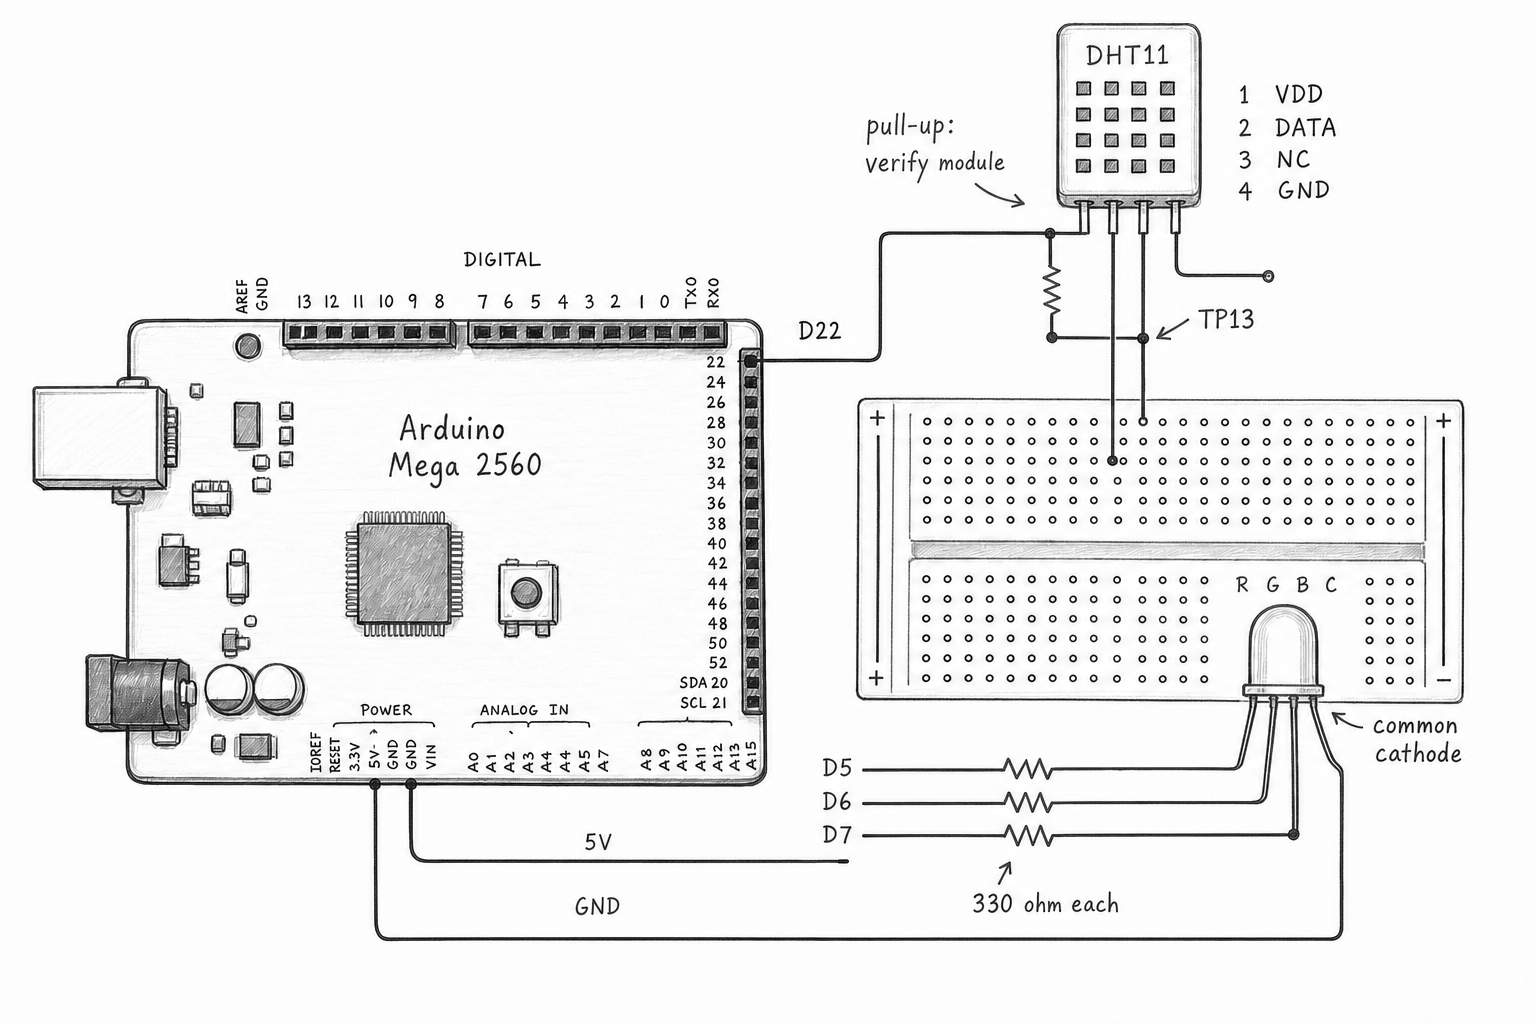
\includegraphics[width=0.96\linewidth]{013-dht11-climate-pencil.png}
  \caption{Pencil orientation of the Mega, DHT11, DATA pull-up, RGB evidence,
  and TP13. This is not an authoritative schematic. Pin placement and
  breadboard connectivity are simplified; use the literal table and the exact
  part documentation. Alternative text: Mega D22 reaches DHT11 DATA and TP13;
  D5, D6, and D7 reach three resistor-limited RGB channels; all parts share
  5\,V and GND while NC remains unconnected.}
\end{figure}

\section{Literal wiring}

\begin{tabularx}{\linewidth}{@{}l l X@{}}
\toprule
Function & Mega connection & Literal path\\
\midrule
DHT11 supply & 5\,V and GND & VDD to 5\,V; GND to GND; never use Vin\\
DATA & D22 & D22 to identified DATA pin; label the sensor-side node TP13\\
NC & none & leave electrically unconnected\\
pull-up & DATA to 5\,V & fit only the value required by the identified part/module\\
red evidence & D5 & D5 through 330\,\(\Omega\) to red anode\\
green evidence & D6 & D6 through 330\,\(\Omega\) to green anode\\
blue evidence & D7 & D7 through 330\,\(\Omega\) to blue anode\\
RGB return & GND & common cathode to GND\\
\bottomrule
\end{tabularx}

Check resistance and continuity with USB removed. Verify that the pull-up does
not become an unintended parallel resistor on a module. Place the meter or
analyzer clip at TP13 while unpowered; inspect the clip spacing before applying
USB power.

\section{Wire transaction}

The adapter drives DATA low only for the request, then releases it:

\[
\text{output low}\rightarrow\text{input/high impedance}\rightarrow
\text{sensor response}\rightarrow 40\text{ data bits}.
\]

\begin{center}
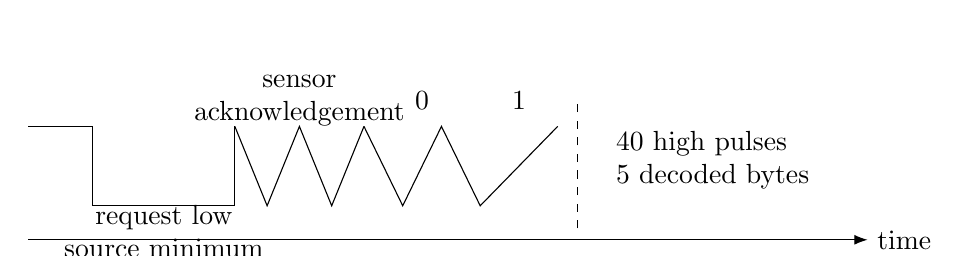
\begin{tikzpicture}[x=0.82cm,y=0.72cm,>=Latex]
  \draw[->] (0,0) -- (13,0) node[right]{time};
  \draw (0,2) -- (1,2) -- (1,0.6) -- (3.2,0.6) -- (3.2,2);
  \node[align=center] at (2.1,0.15) {request low\\source minimum};
  \draw (3.2,2) -- (3.7,0.6) -- (4.2,2) -- (4.7,0.6) -- (5.2,2);
  \node[align=center] at (4.2,2.45) {sensor\\acknowledgement};
  \draw (5.2,2) -- (5.8,0.6) -- (6.4,2) -- (7.0,0.6) -- (8.2,2);
  \node at (6.1,2.45) {0};
  \node at (7.6,2.45) {1};
  \draw[dashed] (8.5,0.2) -- (8.5,2.5);
  \node[align=left] at (10.6,1.4) {40 high pulses\\5 decoded bytes};
\end{tikzpicture}
\end{center}

The drawing shows shape, not measured scale. Record the selected manual's
request, acknowledgement, zero, and one windows before comparing a capture.
Every edge wait has a finite deadline. The five bytes carry humidity,
temperature, and a checksum under the exact selected DHT11 revision. Do not
infer DHT22 compatibility.

\section{Visible state vocabulary}

Color is supporting evidence; pulse count and cadence carry the distinction in
black-and-white observations.

\begin{tabularx}{\linewidth}{@{}l l X@{}}
\toprule
Sample state & D5--D7 indication & Interpretation\\
\midrule
\texttt{Unavailable} & one slow blue pulse & resource owned; first frame pending\\
\texttt{Valid} & steady green & checksum, range, and freshness accepted\\
\texttt{TransportTimeout} & two red pulses & bounded transaction did not complete\\
\texttt{ChecksumFailure} & three red pulses & 40 bits arrived but integrity failed\\
range failure & three red pulses, then amber & decoded value outside limits\\
\texttt{Stale} & steady amber & earlier valid sample exceeded freshness policy\\
setup/evidence failure & indicator off & circuit halted; inspect acquisition separately\\
\bottomrule
\end{tabularx}

TP13 is the primary transport evidence. Predict that released DATA rests high,
observe the request and response, then interpret only whether transport
occurred. A meter can verify the resting level, but a logic analyzer or
oscilloscope is required to inspect pulse timing.

\section{CLI workflow}

\begin{lstlisting}[style=adkcpp]
make host-test-climate-sensor
make host-test-dht11-sensor
make sanitize
make arduino-Lesson013Dht11Climate
make size-check
make lesson-013
make lessons-check

make upload-Lesson013Dht11Climate PORT=/dev/ttyACM0
\end{lstlisting}

Use the repository's actual focused target names if integration reports a
different spelling. Serial is neither required nor used by the canonical
example. Upload and evidence collection remain CLI-driven.

\section{Predict, observe, interpret}

\subsection{Acquisition and first frame}

\textbf{Predict.} Immediately after successful acquisition, one slow pulse
repeats while the adapter honors power-up and acquisition intervals.

\textbf{Observe.} Status cadence: \blank{1.1in}. TP13 resting voltage:
\blank{0.7in}\,V relative to GND. Time to first green: \blank{0.8in}\,s.

\textbf{Interpret.} A waiting pulse proves the software objects initialized.
A high TP13 resting voltage is separate electrical evidence that DATA is
released. Steady green means one sample passed protocol, checksum, range, and
freshness checks.

\subsection{Reversible transport fault}

Remove USB power, disconnect only DATA, inspect the circuit, then restore USB.
Do not short DATA to either rail.

\textbf{Predict.} The bounded transaction times out and two red pulses repeat.

\textbf{Observe.} Pulse count: \blank{0.5in}. Time from request to fault:
\blank{0.8in}. TP13 waveform present? \checkbox\ yes \quad \checkbox\ no.

\textbf{Interpret.} A timeout distinguishes missing wire response from checksum
failure. It does not locate the cause; wiring, part orientation, pull-up, or
sensor health may be responsible.

\subsection{Recovery and freshness}

Remove USB, restore DATA, inspect, then apply USB. A later valid frame should
replace the transport fault normally. To study staleness deterministically,
use the host recorded-sensor test; do not invent an electrical fault that
pretends time advanced.

\textbf{Observe.} Recovery cadence: \blank{1.2in}. Host stale boundary:
\blank{0.8in}\,ms. State at the exact boundary: \blank{1.0in}.

\section{Diagnosis}

\begin{tabularx}{\linewidth}{@{}l X X@{}}
\toprule
Evidence & Likely boundary & Next safe check\\
\midrule
indicator always off & resource or RGB acquisition & remove USB; inspect pins,
resistors, and resource conflicts\\
waiting never ends & power-up interval or no eligible response & inspect TP13
with a bounded capture and confirm the selected part\\
two red pulses & transport timeout & remove USB; inspect DATA continuity,
orientation, supply, and pull-up decision\\
three red pulses & checksum failure & shorten wiring, inspect supply integrity,
and compare measured timing to the selected manual\\
three red then amber & decoded range failure & verify part revision and byte
interpretation; do not present numeric fields as valid\\
steady amber & freshness policy & inspect scheduling and last valid timestamp\\
green but implausible climate & physical accuracy, not transport & compare
against a suitable reference; record uncertainty\\
\bottomrule
\end{tabularx}

\section{Exercises}

\begin{enumerate}
  \item Explain why \texttt{sample(now, freshFor)} must not trigger hardware.
  \item A frame has valid timing but the checksum differs. Which state and
        cadence should appear?

        \blank{2.1in}
  \item A valid sample becomes old. Why must it become \texttt{Stale} rather
        than \texttt{TransportTimeout}?

        \blank{2.5in}
  \item Describe why driving a pulled-up open-style DATA line high is less safe
        than releasing it to input.

        \blank{2.3in}
  \item Choose a freshness interval for a room display and justify it without
        claiming a faster DHT11 acquisition rate.

        \blank{2.0in}
\end{enumerate}

\section{Bench acceptance record}

\textbf{Status before this card is signed: host verified; hardware acceptance
open.} Compilation, tests, and this document do not supply physical evidence.

\begin{tabularx}{\linewidth}{@{}>{\bfseries}l X@{}}
Date / reviewer & \blank{2.7in}\\
Board / USB supply & \blank{2.7in}\\
Sensor or module identity & \blank{2.7in}\\
Primary manual and revision & \blank{2.7in}\\
Pull-up fitted/on module & \blank{2.7in}\\
Measured 5\,V rail & \blank{1.0in}\,V\\
RGB resistor values & red \blank{0.5in}\(\Omega\), green
\blank{0.5in}\(\Omega\), blue \blank{0.5in}\(\Omega\)\\
TP13 released level & \blank{1.0in}\,V relative to GND\\
Request low width & minimum \blank{0.7in}, maximum \blank{0.7in}\\
Acknowledgement widths & low \blank{0.7in}, high \blank{0.7in}\\
Observed zero/one highs & zero \blank{0.7in}, one \blank{0.7in}\\
Reset / shutdown observation & \blank{2.7in}\\
Disconnected-DATA result & \blank{2.7in}\\
Recovery result & \blank{2.7in}\\
Power-removed continuity & \blank{2.7in}\\
Deviations / stop events & \blank{2.7in}\\
\end{tabularx}

\vfill
\evidencebox{\textbf{Acceptance claim.} Resource evidence, released-wire
evidence, successful transport, decoded validity, freshness, and physical
accuracy are separate observations. Sign only the claims actually measured.}

\end{document}
